\chapter{Robotik} % (fold)
\label{cha:robotik}

Die Robotik beschäftigt sich mit der Entwicklung von Robotern, die Aufgaben in verschiedenen Disziplinien bearbeiten können. Neben Disziplinien wie dem Li\-nien\-folgen ist das Erstellen von Karten von Interesse.

\section{Kartierung} % (fold)
\label{sec:kartierung}

Kartierung wird unter anderem in der Rescue League des Robocups eingesetzt. Die Roboter müssen ihre Position im Feld erkennen und eine Karte der Umgebung generieren um zu den \enquote{Opfern} zu gelangen. Allgemein hat die Kartierung in der Robotik eine große Bedeutung, da der Roboter sich in seiner Umgebung zurechtfinden muss. Dabei kann er auf vorbereitete Daten wie z.B. Google Maps zurückgreifen oder selbst seine Position in seiner Umgebung finden und aus dieser eine Karte erstellen. Falls der Roboter auf keine Karte der Umgebung zurückgreifen kann, z.\,B. nach einer Katastrophe, muss er selbst eine Karte seiner Umgebung mit Hilfe der zur Verfügung stehenden Sensoren erstellen und sich in dieser zurechtfinden.\par
Damit die Algorithmen nicht für jeden Roboter neu implementiert werden müssen und für diese eine einheitliche Basis mit wiederverwendbaren Komponenten zur Verfügung steht, hat sich der Einsatz des \ac{ROS} zu einem Standard in der Robotik entwickelt.

% section kartierung (end)

\section{ROS} % (fold)
\label{sec:ros}

\ac{ROS} ist ein auf Linux basierendes Open Source Metabetriebssystem. \ac{ROS} bietet eine \ac{IPC} der teilnehmenden Prozesse durch einen zentralen Master. Dadurch wird die Kommunikation verschiedenartiger Systeme wie z.\,B. Mikrocontroller und Sensoren vereinfacht. \ac{ROS}-Bausteine sind aus Packages aufgebaut. Diese beinhalten alle notwendigen Laufzeitprozesse, sogenannte Nodes, abhängige Bibliotheken und Konfigurationsdateien etc. Durch den Einsatz von Packages wird die Wiederverwendbarkeit der eingesetzten Bausteine gesichert. Diese müssen nun nicht für jeden Roboter neu implementiert werden. \cite{Wiki2018}\par
Nodes sind ausführbare Dateien, aus denen die Funktionsweise des Roboter aufgebaut ist. Mehrere Nodes können über Topics kommunizieren. Hierfür meldet ein Node dem Master, dass er Daten für ein Topic veröffentlichen (publish) will. Falls schon vorher oder erst später ein anderer Node sich für diesen Topic angemeldet (subscribe), informiert der Master beide Nodes über die Existenz des jeweils anderen, damit beide mit dem Datenaustausch beginnen können. Die Daten werden in Form von typisierten Nachrichten (messages) versendet, deren Struktur in einer Textdatei spezifiziert ist. Konsumenten-Nodes erhalten nur Nachrichten falls die selben Messagetypen von Produzenten und Konsumenten verwendet werden. \cite{Wiki2018}\par
Neben dem Publisher-Subscriber-Modell kann ein Node einen Service über einen Namen anbieten. Andere Nodes können nun einen Nachricht an diesen Service senden und eine dafür passende Antwort erhalten. Man spricht von \ac{RPC} Request-Response-Interaktion, da die benutzten Bibliotheken die Aufrufe als \ac{RPC} ermöglichen. Die Services werden wie die Messages in einer Textdatei spezifiziert. \cite{Wiki2018}\par
Ein im Rahmen der Lehrveranstaltung \ac{ROB} für die Kartierung ein\-ge\-setzt\-er, \ac{ROS} nutzender, Roboter ist der Pioneer 3-DX.

% section ros (end)

\section{Pioneer 3-DX} % (fold)
\label{sec:pioneer}

Der Pioneer 3-DX (siehe Abbildung \ref{fig:pioneer}) ist ein zweirädriger, mobiler Roboter mit einem Stützrad. Er besitzt als Aufbau einen Rechner mit Ubuntu, einen Laserscanner für die Kartierung und eine Kinect. Der Roboter wird mittels eines Joysticks über \ac{ROS} gesteuert.

\begin{figure}[!htb]
	\centering
	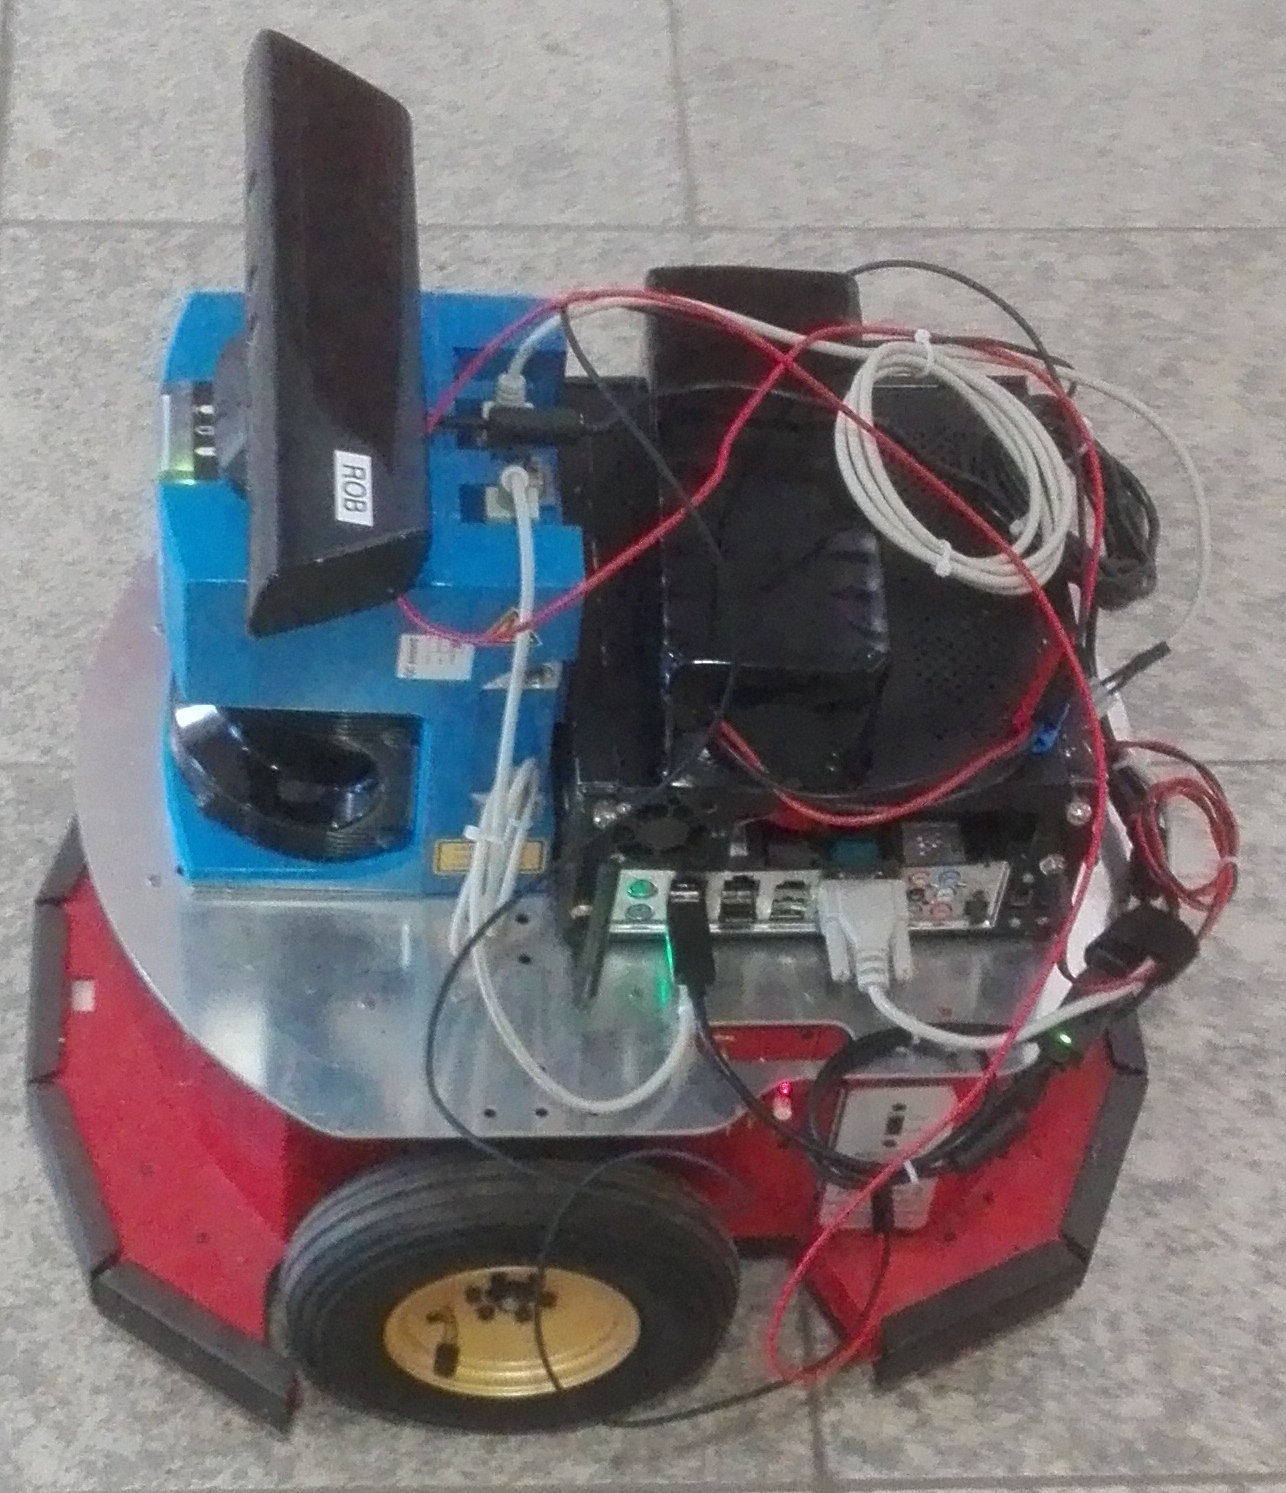
\includegraphics[width=8cm]{pioneer.png}
	\caption{Pioneer 3-DX}
	\label{fig:pioneer}
\end{figure}

Der Pioneer 3-DX kann über eine externe Stromquelle oder Akkus betrieben werden.\par
Während der Vorlesung wurde als Kartierungalgorithmus Grid-Mapping mit Partikelfiltern eingesetzt.\par
Aus der Odometrie des Roboters und den Beobachtungen kann näherungsweise die Karte und die Bewegung des Roboters berechnet werden. Der Roboter setzt hierzu Rao-Blackwellized Partikelfilter ein. Zuerst wird die Trajektorie des Roboters und daraus anschließend die Karte bestimmt. \cite{Grisetti2007}\par
Für die Durchführung der Kartierung werden neben dem Roboter noch einige Packages und Arbeitsschritte benötigt.

% section pioneer (end)

% chapter robotik (end)